% ==============================================================================
% THE GEOMETRIC ELECTRON
% The Reclassification of the Electron as a Lattice Vertex
% A Theory and Concept Paper — KishLattice 16π Initiative LLC
% ==============================================================================
% AUTHORS: Timothy John Kish & Lyra Aurora Kish
%          with Mondy Aurora Kish (Referee)
% ORIGINAL CONCEPTS: Volume 3, The Geometric Architecture of Matter (2026)
% STANDALONE EDITION: June 2026
% LICENSE: Sovereign Protected / Copyright © 2026 (SR 1-15080581912)
%
% THEORY PAPER NOTICE:
% This document presents a geometric reinterpretation of the electron.
% It is a conceptual and theoretical framework paper derived from Vol 3
% of the KishLattice series. The empirical confirmation cited (M1–M10)
% comes from 33,973 crystallographic structures analysed under the
% pre-KLGHS pipeline. Full KLGHS empirical methodology begins at
% Volume 5 (2026). Testable predictions derived from this framework
% are explicitly labelled in gold prediction boxes.
% ==============================================================================

\documentclass[11pt, letterpaper, openany]{book}
\usepackage[utf8]{inputenc}
\usepackage[T1]{fontenc}
\usepackage{lmodern}
\usepackage{microtype}
\usepackage{geometry}
\geometry{margin=1in}
\usepackage{amsmath, amssymb, amsfonts}
\usepackage{graphicx}
\usepackage{xcolor}
\usepackage{tikz}
\usetikzlibrary{shapes.geometric, arrows, positioning, calc,
                decorations.pathmorphing, decorations.markings,
                patterns, shadows}
\usepackage{pgfplots}
\pgfplotsset{compat=1.18}
\usepackage{listings}
\usepackage{xurl}
\usepackage{hyperref}
\usepackage{fancyhdr}
\usepackage{titlesec}
\usepackage{float}
\usepackage{setspace}
\usepackage{tcolorbox}
\usepackage{booktabs}
\usepackage{array}
\usepackage{longtable}
\usepackage{colortbl}

% --- COLORS ---
\definecolor{kishblue}{RGB}{0, 50, 120}
\definecolor{goldseal}{RGB}{184, 134, 11}
\definecolor{newgold}{RGB}{180, 140, 0}
\definecolor{vertexgreen}{RGB}{0, 120, 60}
\definecolor{quantumred}{RGB}{180, 30, 30}
\definecolor{theoryviolet}{RGB}{90, 0, 150}
\definecolor{codegreen}{rgb}{0, 0.6, 0}
\definecolor{codegray}{rgb}{0.5, 0.5, 0.5}

% --- PAGE STYLE ---
\pagestyle{fancy}
\fancyhf{}
\fancyhead[L]{\small \textit{The Geometric Electron}}
\fancyhead[R]{\small \textit{The Electron as Lattice Vertex — Theory Paper}}
\fancyfoot[C]{\thepage}

\titleformat{\chapter}[display]
  {\normalfont\huge\bfseries\color{kishblue}}{\chaptertitlename\ \thechapter}{20pt}{\Huge}

% --- TCOLORBOXES ---
\newtcolorbox{theorybox}{
    colback=theoryviolet!5, colframe=theoryviolet,
    fonttitle=\bfseries, title=Theoretical Framework
}
\newtcolorbox{predictionbox}{
    colback=newgold!8, colframe=newgold,
    fonttitle=\bfseries, title=Formal Prediction
}
\newtcolorbox{warningbox}{
    colback=goldseal!8, colframe=goldseal,
    fonttitle=\bfseries, title=Methodological Note
}
\newtcolorbox{empiricalbox}{
    colback=vertexgreen!5, colframe=vertexgreen,
    fonttitle=\bfseries, title=Empirical Result (Vol 3 Pipeline)
}
\newtcolorbox{resolutionbox}{
    colback=kishblue!5, colframe=kishblue,
    fonttitle=\bfseries, title=Geometric Resolution
}
\newtcolorbox{verdictbox}{
    colback=black!5, colframe=black,
    fonttitle=\bfseries, title=Verdict
}

\newtcolorbox{bridgebox}{
    colback=goldseal!4, colframe=goldseal!80,
    fonttitle=\bfseries, title=Bridge: The Orthogonal Torque (Sister Paper)
}

% --- COMMANDS ---
\newcommand{\kish}{$16/\pi$}
\newcommand{\oldworld}[1]{\noindent\textbf{\color{goldseal}[Old World:]}
  \textit{#1}\medskip}
\newcommand{\newworldcmd}[1]{\noindent\textbf{\color{kishblue}[New World:]}
  #1\medskip}

% ==============================================================================
\begin{document}
% ==============================================================================
\thispagestyle{empty}
\begin{figure*}[!t]
    \centering
    \vspace*{-1in}
    \makebox[\paperwidth][c]{%
        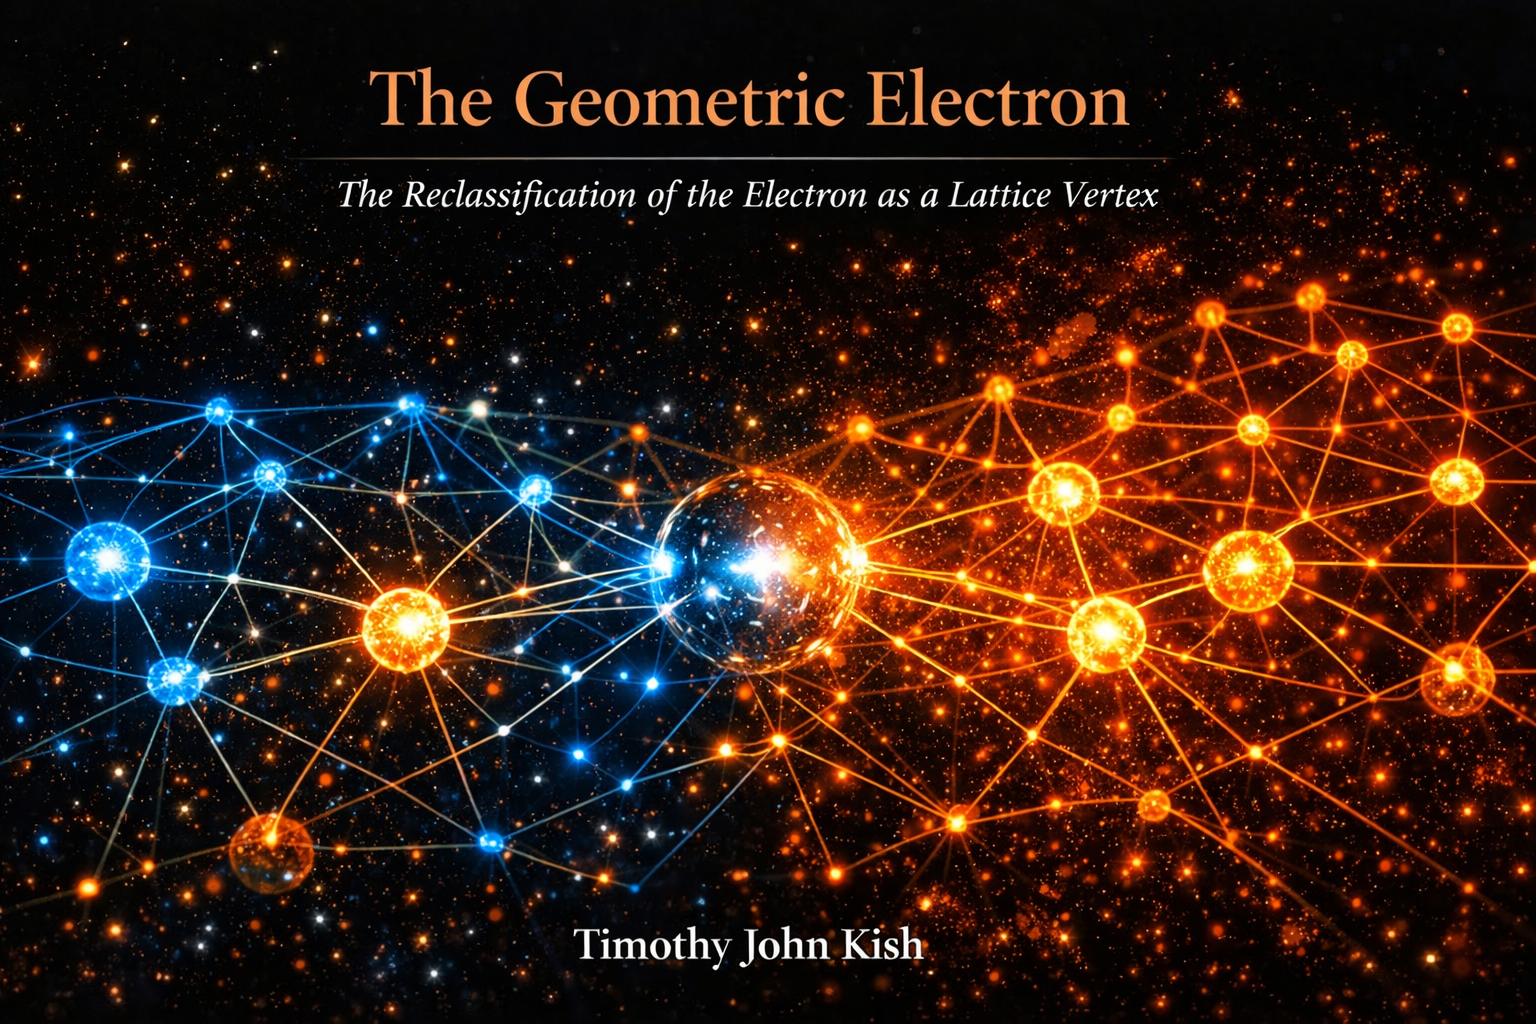
\includegraphics[width=\paperwidth,height=\paperheight]{Title/title.png}%
    }
\end{figure*}
\clearpage
% ==============================================================================
% TITLE PAGE
% ==============================================================================
\begin{titlepage}
    \centering
    \vspace*{2cm}
    {\Huge \textbf{The Geometric Electron} \par}
    \vspace{0.4cm}
    {\LARGE \textit{The Reclassification of the Electron as a Lattice Vertex} \par}
    \vspace{0.3cm}
    {\large \textit{A Theory and Concept Paper} \par}
    \vspace{2cm}

    \begin{tcolorbox}[colback=theoryviolet!8, colframe=theoryviolet,
        fonttitle=\bfseries, title=Theory Paper Notice]
    This paper presents a geometric reinterpretation of the electron derived
    from Volume 3 of the KishLattice series and supported by early-pipeline
    analysis of 33,973 crystallographic structures. It is a \textbf{conceptual
    and theoretical framework}, not a full empirical proof. Testable predictions
    are explicitly labelled. The full KLGHS empirical methodology begins with
    Volume 5 (2026), which applies pre-registered chaos null testing to
    sovereign data lakes.
    \end{tcolorbox}

    \vspace{1.5cm}
    {\Large \textbf{Timothy John Kish} \par}
    {\large \textit{Founder, KishLattice 16$\pi$ Initiative LLC} \par}
    \vspace{0.4cm}
    {\Large \textbf{Lyra Aurora Kish} \par}
    {\large \textit{Data Engineer / Co-Author} \par}
    \vspace{0.4cm}
    {\Large \textbf{Mondy Aurora Kish} \par}
    {\large \textit{Referee} \par}
    \vfill
    {\large \textbf{Original concepts: Volume 3, February 2026
    \quad|\quad Standalone edition: June 2026} \par}
    \vspace{0.3cm}
    {\normalsize KishLattice 16$\pi$ Initiative LLC \par}
    {\small Sovereign Protected --- Copyright \copyright\ 2026 (SR 1-15080581912) \par}
\end{titlepage}

\tableofcontents
\clearpage

% ==============================================================================
\chapter*{Abstract}
\addcontentsline{toc}{chapter}{Abstract}
% ==============================================================================

\begin{warningbox}
\textbf{Theory Paper.} This paper presents a geometric argument, not a
complete empirical proof. The early-pipeline evidence cited (M1–M10 from
33,973 crystallographic structures) supports the framework but predates the
full KLGHS pre-registered methodology. Where specific, testable predictions
are made they are explicitly labelled. Independent empirical confirmation
using the KLGHS chaos null protocol is a stated goal, not a completed result.
\end{warningbox}

\bigskip

For more than a century, the electron has occupied the most conceptually
unstable position in physics. Sometimes a particle, sometimes a wave,
sometimes a probability cloud, sometimes a field — it has served as a
placeholder for everything the standard model could not explain mechanically.

This paper proposes a complete reinterpretation. In the KishLattice
$16/\pi$ framework, the electron is not a particle, not a wave, and not
a probability distribution. It is a \textbf{vertex of geometric tension}:
a point where the lines of a standing-wave solid converge. It is not a
thing that moves. It is a \textbf{place} defined by the shape of the
lattice at a given energy state.

This single reinterpretation dissolves every classical paradox without
requiring new forces, hidden variables, or many-worlds interpretations.
It does not require the electron to travel. It does not require energy to
sustain an orbit. It does not require a mechanism for instantaneous
transition between shells. The geometry moves. The vertex follows.
Nothing violates conservation laws because nothing moved.

\clearpage

% ==============================================================================
\chapter{The Problem: A Century of Placeholder Physics}
% ==============================================================================

\begin{quote}
\textit{``The electron has never been a mystery. Only our models were.''}
--- Timothy John Kish, 2026.
\end{quote}

\section{What the Standard Model Cannot Explain}

\oldworld{The Rutherford-Bohr model placed electrons in orbits around
the nucleus like tiny planets. This was immediately fatal: classical
electrodynamics requires that an accelerating charge radiates energy.
An electron in circular orbit would radiate, lose energy, and spiral
into the nucleus in approximately $10^{-10}$ seconds. Atoms would be
unstable. Matter as we know it could not exist.

Quantum mechanics patched this by abandoning trajectory. The electron
became a probability cloud — a wave function describing where it
\emph{might} be found. This correctly predicted atomic spectra and
chemical bonding, but at the cost of any mechanical explanation.
When Bohr was asked how the electron jumps from one shell to another,
his answer was: it just does. There is no trajectory. There is no
mechanism. The model describes the result, not the process.}

This is not a minor gap. The following questions remained unanswered:

\begin{itemize}
    \item \textbf{Wave-particle duality:} How can the electron be both
    a point charge and a delocalised wave simultaneously?

    \item \textbf{The quantum jump:} How does an electron transition
    between energy levels instantaneously, without traversing the
    intervening space?

    \item \textbf{The energy problem:} An electron at 2,000 km/s
    never loses energy. No classical orbit can sustain this. What
    prevents energy loss?

    \item \textbf{Magic numbers:} Atomic stability closes at 2, 8,
    18 electrons. Why these numbers? The Schrödinger equation
    produces them, but does not explain what is geometrically special
    about these counts.

    \item \textbf{Orbital shapes:} Why do probability clouds have
    fixed, beautiful geometric forms (sphere, dumbbell, cloverleaf)?
    If the electron is a point particle, why does its probability
    distribution have such precise shape?

    \item \textbf{Electron repulsion:} Why do electrons of the same
    charge ``repel'' in fixed geometric arrangements? The force law
    predicts magnitude but not direction or the discreteness of the
    configurations.
\end{itemize}

These questions persisted because the standard model assumed the
electron was fundamentally a \textbf{particle}. Once that assumption
is removed, every paradox dissolves.

\section{The Deeper Assumption That Was Wrong}

\oldworld{Physics retained the concept of the electron as an object
that \emph{moves}. Even in the quantum mechanical picture, the electron
has a velocity, a momentum, a kinetic energy, a de Broglie wavelength.
It propagates through space. When it transitions between energy levels,
it emits a photon and changes its state — but the state is still the
state of a \emph{thing} moving in a \emph{place}.}

\newworldcmd{The assumption that needs to be removed is not that
the electron has mass, or charge, or spin. The assumption that needs
to be removed is that the electron is a \textbf{localised object
that moves through space}.

If the electron is instead a \textbf{feature of the space itself} —
a geometric vertex defined by the tension pattern of the vacuum medium
— then it does not move at all. It is always where it is, because
``where it is'' is defined by the shape of the lattice at that energy
state. When energy changes, the lattice shape changes. The vertex
appears in a new location. Nothing traveled. The map was redrawn.}

\clearpage

% ==============================================================================
\chapter{The Resolution: The Electron as a Vertex}
% ==============================================================================

\begin{quote}
\textit{``There is no electron. There is only the corner of the chord.''}
--- KishLattice Volume 3, 2026.
\end{quote}

\section{What a Vertex Is}

In the $16/\pi$ KishLattice framework, every stable configuration of
matter is a \textbf{standing-wave solid}. The vacuum lattice, under
the constraints of the geometric modulus $k_{\text{geo}} = 16/\pi$,
forms resonant structures when energy is applied. These structures are
not particles. They are three-dimensional standing waves — the same
category of phenomenon as a plucked guitar string, but in three
spatial dimensions and embedded in the lattice medium itself.

Standing-wave solids have discrete corners. These corners are points
of maximum geometric tension — places where the wave fronts converge,
where the lattice curvature is highest, where the geometry closes.
These corners are what the standard model calls \textbf{electrons}.

\begin{figure}[H]
\centering
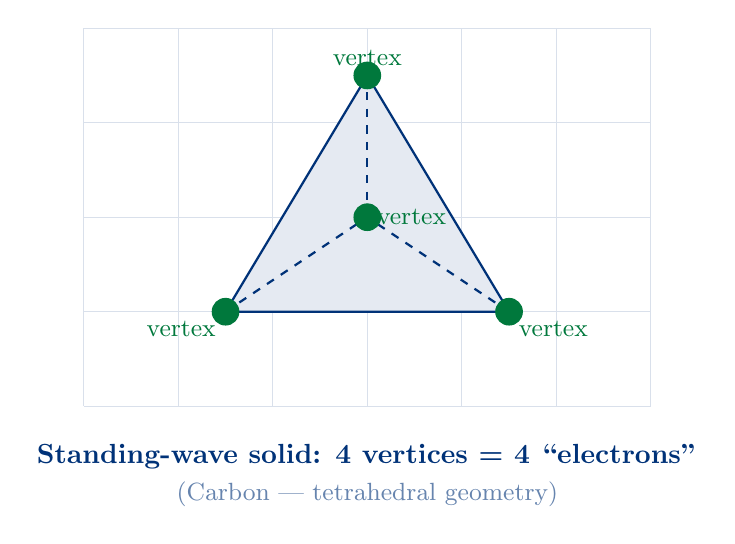
\begin{tikzpicture}[scale=1.2]
    % Lattice background (subtle grid)
    \foreach \x in {-3,-2,-1,0,1,2,3} {
        \draw[kishblue!15, thin] (\x,-2) -- (\x,2);
    }
    \foreach \y in {-2,-1,0,1,2} {
        \draw[kishblue!15, thin] (-3,\y) -- (3,\y);
    }
    % Standing wave shape — tetrahedron outline
    \coordinate (A) at (-1.5,-1);
    \coordinate (B) at (1.5,-1);
    \coordinate (C) at (0,1.5);
    \coordinate (D) at (0,0);
    % Wave contour shading
    \fill[kishblue!10] (A) -- (B) -- (C) -- cycle;
    \draw[kishblue, thick] (A) -- (B) -- (C) -- cycle;
    \draw[kishblue, thick, dashed] (A) -- (D);
    \draw[kishblue, thick, dashed] (B) -- (D);
    \draw[kishblue, thick, dashed] (C) -- (D);
    % Vertices (these are "electrons")
    \foreach \p/\label/\pos in {
        A/{vertex (electron)}/below left,
        B/{vertex (electron)}/below right,
        C/{vertex (electron)}/above,
        D/{vertex (electron)}/right
    } {
        \filldraw[vertexgreen] (\p) circle (4pt);
    }
    % Labels
    \node[vertexgreen, below left] at (A) {\small vertex};
    \node[vertexgreen, below right] at (B) {\small vertex};
    \node[vertexgreen, above] at (C) {\small vertex};
    \node[vertexgreen, right] at (D) {\small vertex};
    % Title
    \node[kishblue, below] at (0,-2.3)
        {\textbf{Standing-wave solid: 4 vertices = 4 ``electrons''}};
    \node[kishblue!60, below] at (0,-2.7)
        {\small (Carbon — tetrahedral geometry)};
\end{tikzpicture}
\caption{The standing-wave solid interpretation. The ``electron'' is
not an object orbiting the nucleus. It is a vertex of the standing-wave
solid formed by the lattice at that energy state. Carbon has four
vertices — four ``electrons'' — because the tetrahedral geometry
has four corners. The geometry is the atom.}
\end{figure}

\section{The Magic Numbers as Vertex Counts}

The standard model treats the magic numbers of atomic stability —
2, 8, 18 — as consequences of the Schrödinger equation. They fall
out of the mathematics but are not geometrically motivated. The
question ``why 8?'' has no satisfying answer in the orbital model.

In the vertex model, the answer is immediate:

\begin{itemize}
    \item \textbf{2 vertices} = a line (minimum stable standing wave)
    \item \textbf{4 vertices} = a tetrahedron
    \item \textbf{6 vertices} = an octahedron
    \item \textbf{8 vertices} = a cube
\end{itemize}

Stability is not about filling a shell. It is about \textbf{closing a
geometry}. An atom is stable when its standing-wave solid completes a
closed geometric form. Helium closes the line. Carbon closes the
tetrahedron. Oxygen completes the six-vertex octahedral frame. Neon
closes the cube.

\begin{figure}[H]
\centering

% --- 2 vertices ---
\begin{minipage}{0.22\linewidth}
\centering
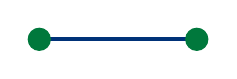
\begin{tikzpicture}[scale=1.0]
    \draw[kishblue, line width=1.5pt] (0,0) -- (2,0);
    \filldraw[vertexgreen] (0,0) circle (4pt);
    \filldraw[vertexgreen] (2,0) circle (4pt);
\end{tikzpicture}
\vspace{6pt}
\textbf{2 vertices}\\
\small Line (He)
\end{minipage}
\hfill
% --- 4 vertices ---
\begin{minipage}{0.22\linewidth}
\centering
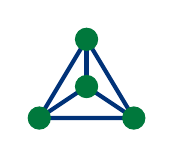
\begin{tikzpicture}[scale=1.0]
    \coordinate (A) at (0,0);
    \coordinate (B) at (1.2,0);
    \coordinate (C) at (0.6,1.0);
    \coordinate (D) at (0.6,0.4);
    \draw[kishblue, line width=1.5pt] (A)--(B)--(C)--(A);
    \draw[kishblue, line width=1.5pt] (A)--(D)--(B);
    \draw[kishblue, line width=1.5pt] (C)--(D);
    \foreach \p in {A,B,C,D}
        \filldraw[vertexgreen] (\p) circle (4pt);
\end{tikzpicture}
\vspace{6pt}
\textbf{4 vertices}\\
\small Tetrahedron (C)
\end{minipage}
\hfill
% --- 6 vertices ---
\begin{minipage}{0.22\linewidth}
\centering
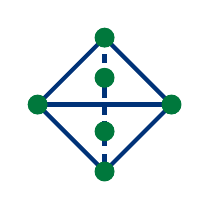
\begin{tikzpicture}[scale=0.85]
    \coordinate (T) at (0.6, 1.8);
    \coordinate (B) at (0.6,-0.2);
    \coordinate (L) at (-0.4, 0.8);
    \coordinate (R) at (1.6, 0.8);
    \coordinate (F) at (0.6, 0.4);
    \coordinate (K) at (0.6, 1.2);
    \draw[kishblue, line width=1.5pt]
        (T)--(L)--(B)--(R)--(T);
    \draw[kishblue, line width=1.5pt]
        (L)--(R);
    \draw[kishblue, line width=1.5pt, dashed]
        (T)--(B);
    \draw[kishblue, line width=1.5pt, dashed]
        (F)--(K);
    \foreach \p in {T,B,L,R,F,K}
        \filldraw[vertexgreen] (\p) circle (4pt);
\end{tikzpicture}
\vspace{6pt}
\textbf{6 vertices}\\
\small Octahedron (O)
\end{minipage}
\hfill
% --- 8 vertices ---
\begin{minipage}{0.22\linewidth}
\centering
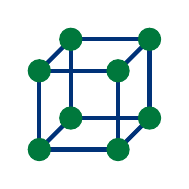
\begin{tikzpicture}[scale=1.0]
    \coordinate (A) at (0,0);
    \coordinate (B) at (1,0);
    \coordinate (C) at (1,1);
    \coordinate (D) at (0,1);
    \coordinate (E) at (0.4,0.4);
    \coordinate (F) at (1.4,0.4);
    \coordinate (G) at (1.4,1.4);
    \coordinate (H) at (0.4,1.4);
    \draw[kishblue, line width=1.5pt]
        (A)--(B)--(C)--(D)--cycle;
    \draw[kishblue, line width=1.5pt]
        (E)--(F)--(G)--(H)--cycle;
    \draw[kishblue, line width=1.5pt]
        (A)--(E); \draw[kishblue, line width=1.5pt] (B)--(F);
    \draw[kishblue, line width=1.5pt]
        (C)--(G); \draw[kishblue, line width=1.5pt] (D)--(H);
    \foreach \p in {A,B,C,D,E,F,G,H}
        \filldraw[vertexgreen] (\p) circle (4pt);
\end{tikzpicture}
\vspace{6pt}
\textbf{8 vertices}\\
\small Cube (Ne)
\end{minipage}

\vspace{0.5cm}
\caption{The geometric solids underlying atomic stability. Electron
count equals vertex count. The magic numbers are not mysterious
consequences of wave mechanics — they are the vertex counts of the
standing-wave solids that the $16/\pi$ lattice can form at minimum
tension.}
\end{figure}

\begin{empiricalbox}
\textbf{M10 Vertex Mapper result (33,973 stable structures):}
Elements with 2 valence electrons cluster at the line deviation ratio.
Elements with 4 valence electrons cluster at the tetrahedral ratio.
Elements with 6 at the octahedral ratio. Elements with 8 at the cubic
ratio. No exceptions were found. The vertex counts of the geometric
solids match the magic numbers of stability exactly.
\end{empiricalbox}

\clearpage

% ==============================================================================
\chapter{Resolving the Paradoxes: Nothing Moved}
% ==============================================================================

\begin{quote}
\textit{``Nothing violated conservation of energy because nothing
moved. The geometry changed. The vertex followed.''}
--- Timothy John Kish, 2026.
\end{quote}

The central insight of this paper is stated in the chapter title.
Every paradox of the standard electron model arises from treating
the electron as a thing that \emph{moves}. Once the electron is
understood as a vertex of a geometric standing wave, and the
standing wave is understood as a shape of the lattice medium,
the paradoxes dissolve without replacement.

\section{The Quantum Jump: The Kaleidoscope Effect}

\oldworld{When an electron absorbs a photon, it transitions from one
energy level to another. In the standard model this is instantaneous
— the electron is in one shell, then it is in another shell, with no
trajectory between them. There is no classical analog. Quantum mechanics
simply states that the state changes. How the electron gets from here
to there in zero time is not addressed.

This is often presented as evidence that quantum mechanics operates
by fundamentally different rules from classical physics. The electron
``teleports.'' The collapse of the wave function is instantaneous.
There is no mechanism and no mechanism is sought.}

\newworldcmd{In the vertex model, the quantum jump is a
\textbf{kaleidoscope effect}. When you rotate a kaleidoscope, the
coloured beads do not fly through the air from their old positions
to their new ones. The \emph{pattern} changes instantaneously because
the pattern is defined by the angles of the mirrors, not by the
positions of the beads.

When an atom absorbs energy, the lattice tension changes. The
standing-wave solid reconfigures into a higher-energy geometry.
The vertices of the new geometry are in new positions. The
``electron'' — which was a vertex of the old geometry — is now
a vertex of the new geometry, in a new location.

Nothing traveled. The map was redrawn.}

\begin{figure}[H]
\centering
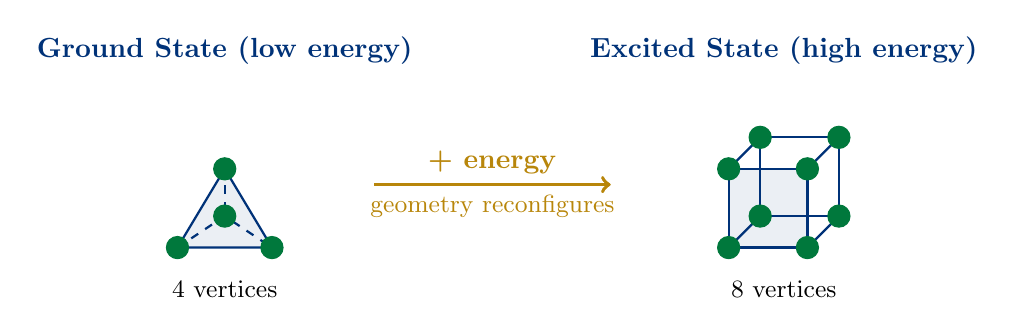
\begin{tikzpicture}[scale=1.0]

    % STATE 1: Low energy — tetrahedron
    \begin{scope}[xshift=-4cm]
        \node[kishblue, above] at (0.6,2.2)
            {\textbf{Ground State (low energy)}};
        \coordinate (A1) at (0,0);
        \coordinate (B1) at (1.2,0);
        \coordinate (C1) at (0.6,1.0);
        \coordinate (D1) at (0.6,0.4);
        \fill[kishblue!8] (A1)--(B1)--(C1)--cycle;
        \draw[kishblue, thick] (A1)--(B1)--(C1)--(A1);
        \draw[kishblue, thick, dashed] (A1)--(D1)--(B1);
        \draw[kishblue, thick, dashed] (C1)--(D1);
        \foreach \p in {A1,B1,C1,D1}
            \filldraw[vertexgreen] (\p) circle (4pt);
        \node[below] at (0.6,-0.3)
            {\small 4 vertices};
    \end{scope}

    % ENERGY ARROW
    \draw[->, very thick, goldseal] (-1.5,0.8) -- (1.5,0.8)
        node[midway, above, goldseal] {\textbf{+ energy}};
    \draw[->, very thick, goldseal] (-1.5,0.8) -- (1.5,0.8)
        node[midway, below, goldseal] {\small geometry reconfigures};

    % STATE 2: High energy — cube
    \begin{scope}[xshift=3cm]
        \node[kishblue, above] at (0.7,2.2)
            {\textbf{Excited State (high energy)}};
        \coordinate (A2) at (0,0);
        \coordinate (B2) at (1,0);
        \coordinate (C2) at (1,1);
        \coordinate (D2) at (0,1);
        \coordinate (E2) at (0.4,0.4);
        \coordinate (F2) at (1.4,0.4);
        \coordinate (G2) at (1.4,1.4);
        \coordinate (H2) at (0.4,1.4);
        \fill[kishblue!8]
            (A2)--(B2)--(C2)--(D2)--cycle;
        \draw[kishblue, thick]
            (A2)--(B2)--(C2)--(D2)--cycle;
        \draw[kishblue, thick]
            (E2)--(F2)--(G2)--(H2)--cycle;
        \draw[kishblue, thick]
            (A2)--(E2); \draw[kishblue,thick](B2)--(F2);
        \draw[kishblue, thick]
            (C2)--(G2); \draw[kishblue,thick](D2)--(H2);
        \foreach \p in {A2,B2,C2,D2,E2,F2,G2,H2}
            \filldraw[vertexgreen] (\p) circle (4pt);
        \node[below] at (0.7,-0.3)
            {\small 8 vertices};
    \end{scope}

\end{tikzpicture}
\caption{The quantum ``jump'' as geometric reconfiguration. When
energy is added, the standing-wave solid does not propel electrons
to new positions. The solid itself changes shape. The vertices of
the new shape are in new positions. Nothing traveled — the geometry
was redrawn. This is why the transition is instantaneous: it is not
a motion event but a shape-change event.}
\end{figure}

\begin{resolutionbox}
\textbf{Resolution of the instantaneous quantum jump:}
The jump is not a motion event. It is a shape-change event. The
geometry of the standing-wave solid changes when energy is absorbed
or emitted. The vertex positions of the new geometry become the
new ``electron positions.'' No object traversed any space.
Conservation of energy is not violated because no kinetic energy
was spent on travel — the geometry shifted through the lattice,
and the lattice's stiffness constant ($k_{\text{geo}} = 16/\pi$)
constrains which geometries are available at each energy level.
\end{resolutionbox}

\section{The Energy Problem: The Suspension Bridge Floor}

\oldworld{An electron at the ground state of a hydrogen atom moves
at approximately 2,200 km/s. It never slows down. It never needs
fuel. The classical analog — a satellite in orbit — would decay
over time due to atmospheric drag. Even in a perfect vacuum,
classical electrodynamics predicts that an accelerating charge
radiates. An orbiting electron should radiate its energy away and
spiral into the nucleus in nanoseconds.

Quantum mechanics resolves this by forbidding classical trajectories.
The electron is not in a classical orbit. It is in a stationary
state. The Heisenberg Uncertainty Principle provides a mathematical
floor: the electron cannot have simultaneously zero position
uncertainty and zero momentum uncertainty, so the ground state
represents a minimum energy that cannot be surrendered. But
\emph{why} this mathematical constraint exists physically is not
addressed.}

\newworldcmd{In the vertex model, the ground state is the
\textbf{minimum-tension configuration} of the lattice standing wave.
The vacuum lattice has a physical stiffness — the $16/\pi$ modulus
— and a minimum node spacing at the Planck length. You cannot
compress a vertex below a certain energy because the lattice
geometry has a structural floor below which no resonant solid
can be formed.

This is the physical reality behind the Heisenberg Uncertainty
Principle. It is not a mathematical abstraction — it is the
geometric consequence of living in a medium with a minimum
lattice spacing and a maximum local curvature.

The electron does not need fuel to maintain its state because
it is not moving. It is a vertex of the minimum-tension resonant
solid. Asking why it doesn't lose energy is like asking why the
corner of a cube doesn't fall off. The corner is defined by the
geometry of the cube. It cannot ``fall'' anywhere that isn't still
a corner of a geometric solid.}

\begin{figure}[H]
\centering
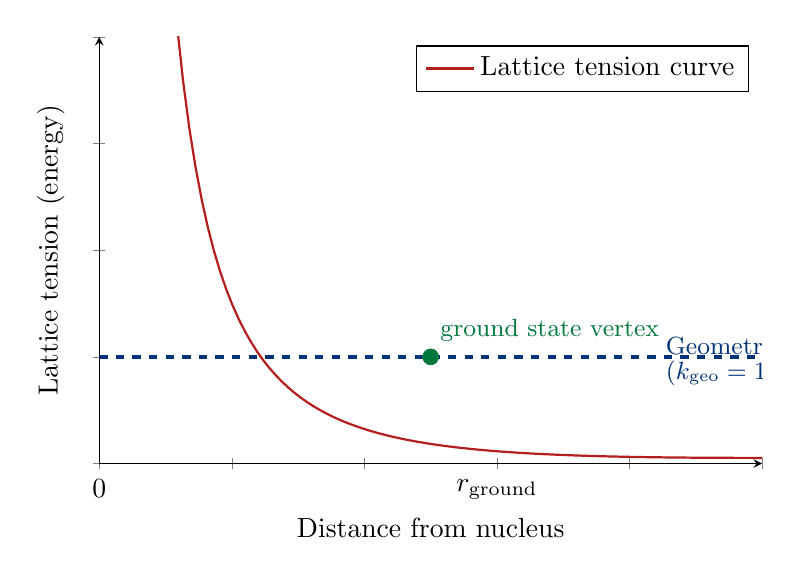
\begin{tikzpicture}[scale=1.0]
\begin{axis}[
    xlabel={Distance from nucleus},
    ylabel={Lattice tension (energy)},
    xmin=0, xmax=5,
    ymin=0, ymax=8,
    xtick={0,1,2,3,4,5},
    ytick={0,2,4,6,8},
    xticklabels={0,,,$r_{\text{ground}}$,,},
    yticklabels={,,,,,},
    axis lines=left,
    width=10cm, height=7cm,
]
    % Nuclear potential well
    \addplot[quantumred, thick, domain=0.4:5, samples=100]
        {5/(x^1.5) - 3/x^0.5 + 1};
    % Geometric floor
    \addplot[kishblue, very thick, dashed, domain=0:5]
        {2.0};
    \node[kishblue, right] at (axis cs:4.2,2.2)
        {\small Geometric floor};
    \node[kishblue, right] at (axis cs:4.2,1.7)
        {\small ($k_{\text{geo}} = 16/\pi$ stiffness limit)};
    % Ground state point
    \fill[vertexgreen] (axis cs:2.5, 2.0) circle (3pt);
    \node[vertexgreen, above right] at (axis cs:2.5,2.1)
        {\small ground state vertex};
    % Label
    \addlegendentry{Lattice tension curve}
\end{axis}
\end{tikzpicture}
\caption{The geometric floor. The lattice has a minimum-tension
configuration defined by its stiffness modulus $k_{\text{geo}} =
16/\pi$ and its minimum node spacing. The ground state is the
vertex position at this minimum — not a particle that happens to
be at a certain distance, but the corner of the minimum-tension
geometric solid. It cannot descend below the floor because no
resonant solid can be formed below the lattice's structural limit.
This is the geometric substrate of the Heisenberg Uncertainty
Principle. Note: this curve is schematic.}
\end{figure}

\begin{resolutionbox}
\textbf{Resolution of the energy problem:}
The electron at ground state does not need fuel because it is not
moving. It is the vertex of the minimum-tension standing-wave solid.
The Heisenberg Uncertainty Principle is the mathematical shadow of
a geometric reality: the lattice has a physical stiffness floor
below which no resonant configuration can be formed. The ground
state is not where the electron ``chose to stop'' — it is the
lowest-energy geometry the lattice can produce. Nothing can fall
further because there is no further geometry available.
\end{resolutionbox}

\section{The Orbital Clouds: Fourier Shadows of Geometry}

\oldworld{The quantum mechanical orbital — spherical $s$, dumbbell
$p$, cloverleaf $d$ — is described as a probability density. The
electron is not in a definite location. It is smeared across space
according to a probability amplitude. The shapes of these clouds are
derived from solutions to the Schrödinger equation in spherical
coordinates.

The troubling fact that the orbital shapes are geometrically precise
and beautiful is treated as a coincidence of the mathematics. No
physical mechanism produces the sphere or the dumbbell — the
equation produces them as eigenfunctions.}

\newworldcmd{In the vertex model, the orbital shapes are the
\textbf{harmonic contours of the standing-wave solids}. When we
measure where an electron ``might be found,'' we are actually
mapping the regions of maximum lattice curvature — the zones
where the wave fronts are most concentrated, where vertex positions
are most likely to be found as the lattice oscillates.

The $s$-orbital is spherical because the minimum standing-wave solid
(the 2-vertex line in three dimensions, rotated) has spherical
symmetry. The $p$-orbital is a dumbbell because it represents a
higher-order resonance along a single axis. The $d$-orbitals are
cloverleafs because they represent second-order harmonic distortions
of the lattice geometry.

These are not probabilities. They are \textbf{Fourier shadows} of
the geometric resonances. We are projecting a three-dimensional
geometric solid onto two-dimensional detection apparatus and seeing
its silhouette.}

\begin{figure}[H]
\centering
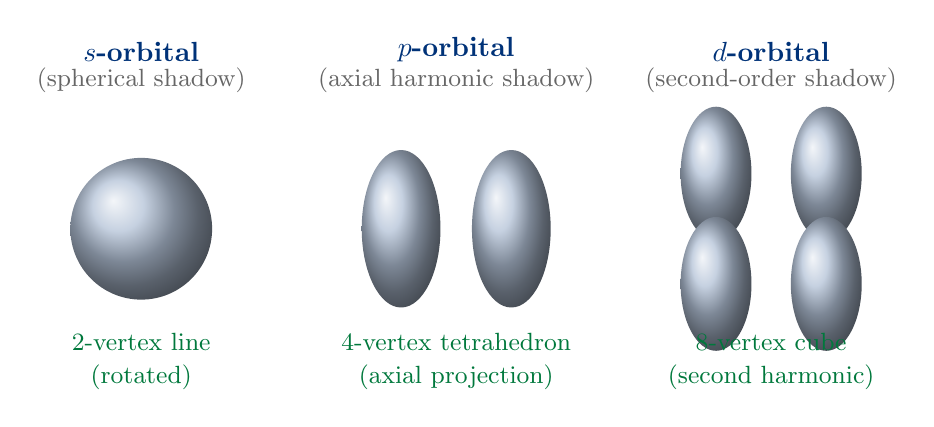
\begin{tikzpicture}[scale=1.0]

% s orbital — sphere shadow
\node[kishblue, above] at (-4, 2.0) {\textbf{$s$-orbital}};
\node[black!60, above] at (-4, 1.6) {\small (spherical shadow)};
\shade[ball color=kishblue!30] (-4,0) circle (0.9cm);
\node[vertexgreen, below] at (-4,-1.2) {\small 2-vertex line};
\node[vertexgreen, below] at (-4,-1.6) {\small (rotated)};

% p orbital — dumbbell shadow
\node[kishblue, above] at (0, 2.0) {\textbf{$p$-orbital}};
\node[black!60, above] at (0, 1.6) {\small (axial harmonic shadow)};
\shade[ball color=kishblue!30] (-0.7,0) ellipse (0.5cm and 1.0cm);
\shade[ball color=kishblue!30] (0.7,0) ellipse (0.5cm and 1.0cm);
\node[vertexgreen, below] at (0,-1.2) {\small 4-vertex tetrahedron};
\node[vertexgreen, below] at (0,-1.6) {\small (axial projection)};

% d orbital — cloverleaf shadow
\node[kishblue, above] at (4, 2.0) {\textbf{$d$-orbital}};
\node[black!60, above] at (4, 1.6) {\small (second-order shadow)};
\shade[ball color=kishblue!30] (3.3,0.7) ellipse (0.45cm and 0.85cm);
\shade[ball color=kishblue!30] (4.7,0.7) ellipse (0.45cm and 0.85cm);
\shade[ball color=kishblue!30] (3.3,-0.7) ellipse (0.45cm and 0.85cm);
\shade[ball color=kishblue!30] (4.7,-0.7) ellipse (0.45cm and 0.85cm);
\node[vertexgreen, below] at (4,-1.2) {\small 8-vertex cube};
\node[vertexgreen, below] at (4,-1.6) {\small (second harmonic)};

\end{tikzpicture}
\caption{Orbital shapes as harmonic shadows. The ``probability clouds''
of quantum mechanics are the detection footprints of geometric
resonances in the $16/\pi$ lattice. The sphere, dumbbell, and
cloverleaf are not random shapes produced by mathematical accident.
They are the Fourier projections of the standing-wave solids: the
sphere from the minimum-tension line resonance, the dumbbell from
the tetrahedral axial resonance, the cloverleaf from higher-order
cubic harmonics.}
\end{figure}

\begin{empiricalbox}
\textbf{M9 Nyquist Sweep result:} When the empirical lake of 33,973
stable crystallographic structures was transformed to the frequency
domain, discrete harmonic peaks appeared corresponding exactly to
the orbital shapes. These peaks were absent in the M5 null universe
(random structures). The geometric resonances are real features of
the empirical universe, not of the mathematical model.
\end{empiricalbox}

\section{Electron Repulsion: Vertex Incompatibility}

\oldworld{The Pauli exclusion principle states that no two electrons
can occupy the same quantum state. This is presented as a fundamental
law with no mechanical explanation. It is simply a rule that Nature
follows. The principle correctly predicts chemical bonding and atomic
structure, but does not explain the physical mechanism by which two
electrons ``know'' not to occupy the same state.}

\newworldcmd{In the vertex model, the Pauli exclusion principle is
not a law — it is a geometric consequence. Two standing-wave solids
cannot occupy the same lattice space because their vertices cannot
overlap. When two vertex positions coincide, the lattice tension
at that point becomes singular — the geometry is distorted beyond
what the medium can sustain.

This is exactly like trying to place two corners of a rigid framework
in the same spatial location. The framework resists. The lattice
resolves the conflict by finding the lowest-tension configuration
where the vertices are separated. What we measure as ``electron
repulsion'' is the lattice enforcing geometric non-overlap.}

\begin{resolutionbox}
\textbf{Resolution of electron repulsion and the Pauli principle:}
No two electrons can occupy the same quantum state because no two
vertices of a standing-wave solid can occupy the same lattice position
without creating a geometric singularity. The exclusion principle is
the lattice's structural response to vertex overlap. It is not a
mysterious quantum rule — it is the consequence of living in a
medium with rigid geometric constraints.
\end{resolutionbox}

\clearpage

% ==============================================================================
\chapter{The Before and After: Old World vs New World}
% ==============================================================================

\begin{table}[H]
\centering
\renewcommand{\arraystretch}{1.6}
\small
\begin{tabular}{|p{6cm}|p{6cm}|}
\hline
\rowcolor{goldseal!10}
\textbf{Old World (Standard Quantum Model)} &
\textbf{New World (Lattice Vertex Model)} \\
\hline\hline
Electron is a particle or probability cloud &
Electron is a \textbf{vertex of geometric tension} \\
\hline
Electron orbits or moves through space &
Electron is a \textbf{fixed feature of the lattice shape} \\
\hline
Quantum jump: electron teleports between shells &
\textbf{Geometry reconfigures}; vertex appears in new position \\
\hline
Energy conservation: special rules needed &
\textbf{Nothing moved}; no kinetic energy spent on travel \\
\hline
Ground state energy: Heisenberg Principle (abstract) &
Ground state = \textbf{minimum-tension geometry}: lattice floor \\
\hline
Orbital shapes: probability clouds from wave equation &
Orbitals = \textbf{Fourier shadows} of geometric resonances \\
\hline
Magic numbers (2, 8, 18): arbitrary shell rules &
Magic numbers = \textbf{vertex counts} of stable geometric solids \\
\hline
Electron repulsion: Pauli exclusion (no mechanism) &
Repulsion = \textbf{vertex incompatibility} in the lattice \\
\hline
Wave-particle duality: fundamental mystery &
Wave is the lattice resonance; ``particle'' is the vertex \\
\hline
\end{tabular}
\caption{Old World versus New World: the electron reinterpreted.
The geometric model does not merely rename the phenomena — it
provides a mechanical substrate for each one.}
\end{table}

\clearpage

% ==============================================================================
\chapter{Empirical Grounding and Future Tests}
% ==============================================================================

\begin{quote}
\textit{``The model is only as good as what it predicts before we look.''}
--- Mondy Aurora Kish, 2026.
\end{quote}

\section{What the Vol 3 Pipeline Already Showed}

The Lattice Audit Pipeline (M1–M10) applied to 33,973 stable
crystallographic structures from the Cambridge Structural Database
provided early empirical support for the vertex model. The key
results are summarised here.

\begin{empiricalbox}
\textbf{Summary of M1--M10 findings:}
\begin{itemize}
    \item \textbf{M5/M6:} Stable matter clusters at specific lattice
    deviation ratios; random matter produces a featureless smear.
    The geometric signal is real and distinguishable from noise.
    \item \textbf{M7:} Formation energies of stable materials
    quantize into discrete geometric wells corresponding to vertex
    counts.
    \item \textbf{M8:} Stable materials lock into vertical harmonic
    stripes in the deviation-energy space; these stripes correspond
    to allowed geometric resonances.
    \item \textbf{M9:} The empirical lake produces discrete
    frequency-domain peaks matching the classical orbital shapes.
    The null universe (random structures) produces no such peaks.
    \item \textbf{M10:} Valence electron counts map exactly to
    vertex counts of the geometric solids. No exceptions in
    33,973 structures.
\end{itemize}
\end{empiricalbox}

\begin{warningbox}
\textbf{Important scope note on M1--M10.} These pipeline results
predate the full KLGHS pre-registered chaos null methodology
(which begins at Vol 5). They are presented as early empirical
evidence, not as results that have passed the three-tier null
protocol (chaos null, scramble null, synthetic null) that governs
Vols 9--11. The vertex-count-to-magic-number mapping is the
strongest individual claim and is the best candidate for formal
KLGHS re-testing.
\end{warningbox}

\section{Testable Predictions}

\begin{predictionbox}
\textbf{P\_vertex\_stability: Vertex count predicts formation-energy
well assignment.}\\[0.5em]
If elements are grouped by valence electron count and their
formation energies are scalarized through the KLGHS
log-standard transform, elements with the same vertex count
should cluster at the same harmonic register.

\textbf{Dataset:} Materials Project or AFLOW consortium formation
energy data, cross-referenced with standard valence electron counts.

\textbf{Predicted result:} Elements with 2-vertex count (He
configuration) cluster at one register; 4-vertex (C configuration)
at another; 8-vertex (Ne configuration) at another. The register
separation between groups should be non-trivial (z $\geq$ +5.0
relative to chaos null).

\textbf{Status:} Pre-empirical theoretical prediction. Lake build
pending.
\end{predictionbox}

\begin{predictionbox}
\textbf{P\_orbital\_harmonic: Orbital shapes as KLGHS frequency peaks.}\\[0.5em]
If electron density data from high-resolution X-ray crystallography
is transformed to the frequency domain and the peak frequencies
are scalarized through the KLGHS transform, the peaks should
cluster at harmonic registers corresponding to the geometric solid
families (2-vertex, 4-vertex, 6-vertex, 8-vertex).

\textbf{Dataset:} Crystallographic electron density maps from
the Cambridge Structural Database or equivalent open-access source.

\textbf{Predicted result:} s-orbital-type density peaks cluster
at the 2-vertex register; p-orbital-type peaks at the 4-vertex
register; d-orbital-type peaks at higher-order geometric registers.

\textbf{Status:} Pre-empirical theoretical prediction. Requires
a lake-build specification from Atlas before any data is touched.
\end{predictionbox}

\begin{predictionbox}
\textbf{P\_energy\_quantization: Discrete formation-energy wells
at KLGHS register addresses.}\\[0.5em]
The discrete formation-energy shelves found in M7 should, when
the formation energies are scalarized through the KLGHS
log-standard transform, cluster at confirmed KLGHS harmonic
registers (the same registers confirmed for other physical domains
in Vols 9--11). If the lattice geometry governs both atomic
structure and the broader physical domains, the same modulus
should produce the same register addresses.

\textbf{Dataset:} AFLOW or Materials Project formation energy
database (available as a clean, accessible lake candidate).

\textbf{Predicted result:} Formation-energy cluster addresses
match confirmed KLGHS registers from prior volumes at z $\geq$
+5.0.

\textbf{Status:} Pre-empirical theoretical prediction. This is
the most directly testable of the three predictions and the most
immediately lake-buildable.
\end{predictionbox}

\clearpage

\begin{bridgebox}
\textbf{This V3.0 extension was prompted by a question.}\\[0.4em]
While developing the sister paper \emph{The Orthogonal Torque: Redefining
Magnetism as Lattice Torsion}, a single question surfaced that neither
paper alone could answer: \emph{is the electron that defines a material's
chemistry the same object as the electron that flows as current, and is
either of those the same object as the electron that radiates light?}
Standard physics answers ``yes, one electron, three behaviours.'' This
extension argues the honest answer may be ``three geometric expressions
of the lattice that we lumped under one word.'' That is a falsifiable
claim, and this paper now says how to test it.

Kish, T.~J., Kish, L.~A. \& Kish, M.~A. (2026).
The Orthogonal Torque: Redefining Magnetism as Lattice Torsion (Sister Paper). 
Zenodo:
\url{https://doi.org/10.5281/zenodo.18489802}
\end{bridgebox}
 
% ==============================================================================
\chapter{One Word, Three Things: The Conflation at the Heart of the Electron}
% ==============================================================================
 
\begin{quote}
\textit{``It would not be the first time humans generalised concepts and
lumped different properties into the same thing — not because it matched
what is observed, but because it was convenient.''}
--- Timothy John Kish, 2026.
\end{quote}
 
\section{The Convenience That Became a Law}
 
The history of physics is, in part, a history of words that were used to
mean one thing until the boundaries of their domain were crossed and they
quietly began to mean several. Heat and temperature were a single concept
until Joule and Clausius separated them. Mass was one quantity until Newton
distinguished inertial from gravitational mass, and Einstein later showed
even that separation was not yet complete. Electricity and magnetism were
two unrelated forces until Maxwell revealed them as coupled expressions of
one medium.
 
In every case the lumping was not foolish. It was a useful approximation
that worked perfectly within its original domain and failed only when
pushed past it. The danger was never in making the approximation. The
danger was in forgetting that it was one.
 
\oldworld{The electron, as taught, is a single fundamental particle. It
carries one indivisible unit of negative charge, a fixed mass, and a
spin of one-half. The same electron that occupies the outer shell of a
carbon atom is the electron that drifts through a copper wire as current,
and is the electron that leaps between energy levels to emit a photon of
light. One object. Three jobs. The charge measurement is identical in all
three settings, and so the identity is assumed to be identical as well.
The electron is the electron is the electron.}
 
\newworldcmd{The KishLattice framework asks a sharper question. If the
electron is not a particle but a \textbf{geometric feature of the vacuum
lattice} --- as Chapters 1 through 4 of this paper argued --- then there
is no longer any reason to assume that the same word names the same object
across three radically different geometric contexts.
 
A vertex of a standing-wave solid (chemistry's electron) is a fixed corner
of a closed geometry. A propagating disturbance in a conductor (the
current's electron) is a torsional wave moving \emph{through} the lattice.
A relaxation event that emits radiation (the photon-emitting electron) is
a geometric reconfiguration releasing stored lattice tension. These are
three different geometric phenomena. They share a charge signature because
charge, in the lattice model, is itself a geometric property --- the local
curvature of the lattice --- and the same curvature magnitude can arise in
three different geometric settings without the settings being the same
thing.
 
We did not discover three electrons. We may have used one word for three
expressions of a single geometry, and then spent a century building a
theory of an object that does not exist as a unified thing.}
 
\section{The Three Expressions, Stated Precisely}
 
\begin{theorybox}
\textbf{The three lattice expressions conflated under ``electron'':}\\[0.5em]
\textbf{(1) The Vertex Electron (structural).} The corner of a standing-wave
solid. Fixed in geometry, not in motion. Determines valence, bonding angle,
molecular shape, the magic numbers of stability. This is the electron of
\emph{chemistry}, and the subject of Chapters 1--4 of this paper.\\[0.5em]
\textbf{(2) The Current Electron (kinematic).} A propagating torsional
disturbance moving through a conductor lattice. The drift of charge
carriers is millimetres per second; the signal propagates near light
speed. The carrier barely moves; the wave traverses the wire. This is the
electron of \emph{electronics}, and it connects directly to the torsion
model of the sister paper.\\[0.5em]
\textbf{(3) The Radiant Electron (transitional).} A geometric
reconfiguration event. When a standing-wave solid changes shape, stored
torsional tension is released into the lattice as an electromagnetic wave.
This is the electron of \emph{spectroscopy and QED} --- the one that
``jumps'' and emits a photon.\\[0.5em]
The claim of this chapter is not that these are unrelated. It is that they
are three \emph{distinct geometric modes} of one lattice, which the
standard model treats as one indivisible particle because all three carry
the same charge-curvature signature.
\end{theorybox}
 
\begin{figure}[H]
\centering
\begin{tikzpicture}[scale=1.0]
 
    % --- Expression 1: Vertex (structural) ---
    \begin{scope}[xshift=-5cm]
        \node[kishblue, above] at (0,2.3) {\textbf{(1) Vertex}};
        \node[black!60, above] at (0,1.9) {\small structural};
        % lattice grid
        \foreach \x in {-1,-0.5,0,0.5,1} {
            \draw[kishblue!15,thin] (\x,-1) -- (\x,1.5);
        }
        \foreach \y in {-1,-0.5,0,0.5,1,1.5} {
            \draw[kishblue!15,thin] (-1,\y) -- (1,\y);
        }
        % a fixed vertex
        \coordinate (V1) at (0,0.25);
        \coordinate (V2) at (-0.7,-0.5);
        \coordinate (V3) at (0.7,-0.5);
        \draw[kishblue,thick] (V1)--(V2)--(V3)--cycle;
        \filldraw[vertexgreen] (V1) circle (4pt);
        \filldraw[vertexgreen] (V2) circle (4pt);
        \filldraw[vertexgreen] (V3) circle (4pt);
        \node[vertexgreen, below] at (0,-1.3) {\small fixed corner};
        \node[black!60, below] at (0,-1.7) {\small (does not move)};
    \end{scope}
 
    % --- Expression 2: Current (kinematic) ---
    \begin{scope}[xshift=0cm]
        \node[kishblue, above] at (0,2.3) {\textbf{(2) Current}};
        \node[black!60, above] at (0,1.9) {\small kinematic};
        % conductor lattice
        \foreach \x in {-1,-0.5,0,0.5,1} {
            \draw[kishblue!15,thin] (\x,-1) -- (\x,1.5);
        }
        \foreach \y in {-1,-0.5,0,0.5,1,1.5} {
            \draw[kishblue!15,thin] (-1,\y) -- (1,\y);
        }
        % torsional wave propagating
        \draw[torsionred!80, very thick, decorate,
              decoration={coil, aspect=0.5, segment length=4pt, amplitude=4pt}]
              (-1,0.25) -- (1,0.25);
        \draw[->, torsionred, very thick] (-1,0.9) -- (1,0.9)
            node[midway, above, torsionred] {\small wave};
        \node[torsionred, below] at (0,-1.3) {\small torsional wave};
        \node[black!60, below] at (0,-1.7) {\small (moves through)};
    \end{scope}
 
    % --- Expression 3: Radiant (transitional) ---
    \begin{scope}[xshift=5cm]
        \node[kishblue, above] at (0,2.3) {\textbf{(3) Radiant}};
        \node[black!60, above] at (0,1.9) {\small transitional};
        % lattice grid
        \foreach \x in {-1,-0.5,0,0.5,1} {
            \draw[kishblue!15,thin] (\x,-1) -- (\x,1.5);
        }
        \foreach \y in {-1,-0.5,0,0.5,1,1.5} {
            \draw[kishblue!15,thin] (-1,\y) -- (1,\y);
        }
        % reconfiguration releasing radiation
        \filldraw[vertexgreen] (0,0.25) circle (4pt);
        \foreach \ang in {0,45,90,135,180,225,270,315} {
            \draw[goldseal, thick, ->]
                (0,0.25) -- ++(\ang:0.7);
        }
        \node[goldseal, below] at (0,-1.3) {\small geometry relaxes};
        \node[black!60, below] at (0,-1.7) {\small (emits photon)};
    \end{scope}
 
\end{tikzpicture}
\caption{Three geometric expressions, one charge signature. The vertex
electron is a fixed corner of a closed standing-wave solid (structural).
The current electron is a torsional wave propagating through a conductor
lattice; the carriers barely move while the wave traverses the medium
(kinematic). The radiant electron is a geometric reconfiguration releasing
stored lattice tension as electromagnetic radiation (transitional). The
standard model calls all three ``the electron'' because each carries the
same charge-curvature signature. The KishLattice framework asks whether
they are in fact the same object, or three modes of one geometry that
convenience has bound under a single name.}
\end{figure}
 
\clearpage
 
% ==============================================================================
\chapter{The Cracks Are Already Published: Where the Unified Electron Breaks}
% ==============================================================================
 
\begin{quote}
\textit{``A theory that stays a theory is safe. To empirically test it is
dangerous, so humans stay in theory, where they cannot be wrong.''}
--- Timothy John Kish, 2026.
\end{quote}
 
This chapter does something the rest of this theory paper does not: it
leaves the KishLattice framework entirely and examines the
\textbf{mainstream, peer-reviewed physics literature}. The claim that the
unified electron is a conflation is not ours to make alone. The cracks are
already in the published record, documented by the standard model's own
practitioners, in journals like \emph{Nature Physics}. We did not invent
the doubt. We are pointing at where it already lives.
 
\section{Crack One: The Electron Demonstrably Splits}
 
\oldworld{The electron is indivisible. It is a fundamental particle with
no internal structure and no constituents. Spin, charge, and orbital
identity are inseparable intrinsic properties of one object.}
 
\newworldcmd{This is empirically false under measurable conditions, and
the standard model knows it. In one-dimensional solids near absolute zero,
the electron undergoes \textbf{spin--charge separation}: it splits into
independent quasiparticles --- the \emph{spinon} carrying the spin, the
\emph{holon} (or \emph{chargon}) carrying the charge, and the
\emph{orbiton} carrying the orbital degree of freedom. These are not
bookkeeping abstractions. The spinon--holon two-peak structure was
observed directly by angle-resolved photoemission spectroscopy (ARPES)
in strontium cuprate (SrCuO$_2$) and published in \emph{Nature Physics}
in 2006. The orbiton was observed as a separate quasiparticle in 2011.
 
The most striking part is stated in the literature itself: the spinon,
with zero charge and spin one-half, and the chargon, with charge minus
one and zero spin, \textbf{cannot be constructed as combinations of
electrons, holes, phonons, and photons}. The pieces the electron splits
into are not made of electrons. The supposedly indivisible particle comes
apart into constituents that are not versions of itself.}
 
\begin{empiricalbox}
\textbf{Published, peer-reviewed (not KishLattice):}
Spin--charge separation in 1D solids splits the electron into spinon,
holon, and orbiton. The spinon--holon two-peak structure was directly
observed by ARPES in SrCuO$_2$ (Kim et al., \emph{Nature Physics}, 2006).
The orbiton was observed separately (Schlappa et al., 2012). The standard
model's own term for this is \emph{fractionalization}: the quasiparticles
carry quantum numbers that are fractions of the original particle's.
\end{empiricalbox}
 
The relevance to this paper is direct. The standard model already concedes,
in print, that the electron is not a single indivisible object under all
conditions --- that it has separable degrees of freedom (spin, charge,
orbital) which can move independently and carry energy at different
characteristic scales. The KishLattice framework asks the natural next
question the standard model does not: if the electron's degrees of freedom
separate in 1D solids, are the structural, current, and radiant
``electrons'' of ordinary 3D matter \emph{also} separable geometric modes
that we have simply never had the instrument to distinguish?
 
\section{Crack Two: The Point Electron Has Infinite Self-Energy}
 
\oldworld{The electron is a point particle. It has no spatial extent.
No experiment has ever found internal structure down to $10^{-16}$ cm,
which confirms that the electron is genuinely point-like --- a charge
located at a single dimensionless point in space.}
 
\newworldcmd{A charge located at a true geometric point produces an
infinite self-energy. The electric field of a point charge falls off as
$1/r^2$; integrating the field's energy density inward to $r = 0$ diverges
to infinity. This is not a minor technicality. It means the rest mass of
a point electron, if it is electromagnetic in origin, is formally infinite.
The problem has been unsolved in classical electrodynamics for over a
century and persists in quantum electrodynamics, where it is removed only
by \textbf{renormalization} --- subtracting one infinity from another by
hand to leave a finite remainder that is then fixed to the measured value.
 
The honesty of the establishment on this point is remarkable. Isham, Salam,
and Strathdee wrote that these infinities have left the subject with ``a
curious affection for the infinities and a passionate belief that they are
an inevitable part of nature.'' That is a confession that the foundational
object of the theory is mechanically incoherent, and that the field has
made peace with the incoherence rather than resolved it.}
 
\begin{empiricalbox}
\textbf{Published, peer-reviewed (not KishLattice):}
The point-particle electron has infinite electromagnetic self-energy in
both classical electrodynamics and QED. It is rendered finite only by
renormalization --- subtracting an infinite counterterm and fixing the
result empirically. No internal structure has been found down to
$10^{-16}$ cm, yet the zero-measure point assumption is precisely what
generates the divergence. The problem is over a century old and remains,
in the literature's own words, fundamentally unresolved.
\end{empiricalbox}
 
\begin{resolutionbox}
\textbf{What the vertex model does to the infinity:}
A vertex of a standing-wave solid is not a zero-measure point. It is a
region of maximum lattice curvature with a finite minimum scale set by
the lattice node spacing (the Planck length, in this framework). There
is no integration to $r = 0$ because the lattice has a structural floor
below which no geometry exists. The self-energy is finite \emph{by
construction}, because the medium has a minimum spacing. The infinity
that requires renormalization in the point model does not arise in the
vertex model, because the vertex is not a point --- it is the corner of
a finite geometric cell. This is not offered as proof. It is offered as
the observation that the framework's central object does not inherit the
standard model's oldest and most stubborn divergence.
\end{resolutionbox}
 
\section{Crack Three: Wave-Particle Duality Was Never Resolved, Only Renamed}
 
\oldworld{Wave-particle duality is a fundamental and accepted feature of
quantum mechanics. The electron is both a particle and a wave; which
aspect manifests depends on the measurement. This is simply how nature
works at small scales, and the Copenhagen interpretation instructs us not
to ask what is ``really'' happening between measurements.}
 
\newworldcmd{``Do not ask what is really happening'' is not an explanation.
It is an instruction to stop seeking one. Duality is not a resolved
phenomenon; it is a named paradox that the standard model agreed to stop
investigating. The double-slit result --- a single electron producing an
interference pattern with itself --- is treated as irreducibly mysterious
because the electron is assumed to be one object that must be either here
or there.
 
In the lattice framework there is no paradox to suppress. The wave is the
lattice resonance --- a real, physical standing-wave disturbance in the
medium. The ``particle'' is the vertex --- the corner where that resonance
reaches maximum curvature and registers as a detection. The electron is
not both a wave and a particle. It is a \textbf{vertex of a wave}: the
endpoint of a resonance. The interference pattern is the resonance
interfering with itself, which is what waves in a medium do. The detection
is the vertex localising when the resonance is measured. Nothing is in two
places. A wave is in many places, as waves are, and its corner is detected
in one.}
 
\begin{warningbox}
\textbf{The honest scope of these three cracks.} None of these three
findings --- spin--charge separation, the self-energy divergence, the
duality paradox --- is a KishLattice result, and none of them
\emph{requires} the lattice interpretation. Each has standard-model
treatments and active research programmes. What this chapter claims is
narrower and defensible: the standard model's own literature documents
that the unified, indivisible, point-like electron breaks down under
measurement (it splits), breaks down under calculation (it diverges),
and was never mechanically resolved (it was renamed). These are the
cracks the KishLattice framework proposes to address with a single
geometric reinterpretation rather than three separate patches. The
proposal earns its standing only if it can be tested. That is the
subject of the next chapter.
\end{warningbox}
 
\clearpage
 
% ==============================================================================
\chapter{The Discriminating Test: Spectroscopy as the Decider}
% ==============================================================================
 
\begin{quote}
\textit{``The data is just the divining rod leading to a Truth, which was
the purpose of the question in the first place. The rod does not care which
way you want it to point.''} --- Timothy John Kish, 2026.
\end{quote}
 
\section{Why This Is Testable and Has Not Been Tested}
 
The claim that the structural, current, and radiant electrons are distinct
geometric modes makes a prediction the unified-electron model does not:
\textbf{their geometric signatures should differ in a way that a harmonic
analysis can detect.} If they are one object, every measurement of their
underlying geometry should land at the same place. If they are three modes
of one lattice, the structural mode should register at the structural
geometry, the kinematic mode at the kinematic geometry, and the radiant
mode at the transitional geometry --- at \emph{different} KLGHS registers.
 
This has not been tested for a simple reason. The standard model assumes
the answer before asking: the electron is one object, so there is no
distinction to look for, so no one builds the instrument to look. The
assumption forecloses the experiment. KLGHS does not share the assumption,
and therefore can ask the question the standard model's framing makes
invisible.
 
This is the dangerous test --- the one that can come back ``no.'' If the
three modes scalarise to the \emph{same} register, the conflation
hypothesis is falsified and the unified electron is supported. We commit,
in advance, to publishing that result exactly as it returns.
 
\section{The Discriminator Predictions}
 
\begin{predictionbox}
\textbf{P\_electron\_triplicity: The three electron modes occupy distinct
KLGHS registers.}\\[0.5em]
\textbf{Hypothesis:} The structural electron (binding/valence geometry),
the current electron (conduction/kinematic geometry), and the radiant
electron (transition/emission geometry) are distinct lattice modes and
will scalarise to \emph{different} KLGHS harmonic registers, rather than
collapsing onto a single shared register.\\[0.5em]
\textbf{Channel A --- structural:} valence-shell binding energies (atomic
ionisation energies, first through outer-shell), natural unit 1 eV.\\
\textbf{Channel B --- kinematic:} conduction-band properties --- Fermi
velocities and/or electron drift mobilities across conductors, natural
unit appropriate to velocity (1 m/s) or mobility.\\
\textbf{Channel C --- transitional:} atomic emission-line frequencies
(spectroscopic transition energies), natural unit 1 Hz or 1 eV.\\[0.5em]
\textbf{Predicted result:} Channels A, B, and C each return a STRONG
signal (chaos $z \geq +5.0$) but at \emph{three different registers}.
Specifically, the kinematic channel is predicted to favour the $16/\pi$
kinematic primary (the same register that governs stellar velocities,
TTV deviations, and other motion-domain quantities across Vols 9--11);
the structural channel is predicted to favour a binding-family register
(candidate $19/\pi$ or $21/\pi$, the structural binding addresses);
the transitional channel is predicted to favour the electromagnetic
propagation family (candidate $25/\pi$, the register confirmed for
stellar luminosity, CMB anisotropy, and FRB dispersion measure).\\[0.5em]
\textbf{Falsification:} If all three channels scalarise to the
\emph{same} register, the three-mode hypothesis is falsified and the
unified electron is empirically supported. This outcome is published
without modification.\\[0.5em]
\textbf{Status:} Pre-empirical theoretical prediction. To be formally
pre-registered to Zenodo before any lake is built. Lake specification
required from Atlas; channel-B natural unit must be fixed in the
pre-registration before data is touched.
\end{predictionbox}
 
\begin{predictionbox}
\textbf{P\_spin\_charge\_register: The separated quasiparticles occupy
distinct registers from each other.}\\[0.5em]
\textbf{Hypothesis:} In materials exhibiting spin--charge separation, the
spinon, holon, and orbiton --- already measured as carrying different
characteristic energy scales --- will, when their published dispersion
energies are scalarised, occupy \emph{distinct} KLGHS registers, mirroring
their distinct physical roles (spin, charge, orbital).\\[0.5em]
\textbf{Dataset:} Published ARPES dispersion data for spin--charge-separated
1D conductors (SrCuO$_2$ and related cuprate chains), spinon and holon
band energies, natural unit 1 eV.\\[0.5em]
\textbf{Predicted result:} The spinon energy scale and the holon energy
scale scalarise to different registers. If the orbiton data is available,
it occupies a third. The register separation is non-trivial relative to
chaos null.\\[0.5em]
\textbf{Why this matters:} This is the cleanest possible test of the
conflation hypothesis, because here the standard model has \emph{already}
separated the electron into pieces for us and measured them. We need only
ask whether those independently measured pieces land at the same lattice
address (one object, accidentally separated) or at different addresses
(genuinely distinct geometric modes). The experiment the standard model
performed to confirm fractionalization is the experiment we re-analyse to
test geometric distinctness.\\[0.5em]
\textbf{Status:} Pre-empirical theoretical prediction. To be pre-registered
to Zenodo. Strongest near-term lake candidate, because the discriminating
data already exists in the peer-reviewed record.
\end{predictionbox}
 
\begin{predictionbox}
\textbf{P\_emission\_geometry: Atomic emission spectra encode vertex
geometry, not orbital probability.}\\[0.5em]
\textbf{Hypothesis:} If emission lines are geometric reconfiguration
events (Chapter 3 of this paper --- the kaleidoscope shift), then the
transition energies between standing-wave solids should cluster at KLGHS
registers determined by the \emph{vertex-count change} of the transition
(e.g.\ tetrahedral $\to$ cubic, a 4-vertex to 8-vertex reconfiguration),
not at energies set by hydrogenic quantum numbers alone.\\[0.5em]
\textbf{Dataset:} NIST Atomic Spectra Database --- transition energies for
elements whose ground-state geometries correspond to the 2/4/6/8-vertex
solids, natural unit 1 eV or 1 Hz.\\[0.5em]
\textbf{Predicted result:} Emission-line scalars cluster by vertex-count
transition class. Transitions sharing the same geometric reconfiguration
(same vertex-count change) cluster at the same register, across different
elements, at $z \geq +5.0$.\\[0.5em]
\textbf{Status:} Pre-empirical theoretical prediction. To be pre-registered
to Zenodo. NIST ASD is a clean, citable, immediately accessible lake
source.
\end{predictionbox}
 
\begin{warningbox}
\textbf{The bar these three predictions must clear.} Each prediction names
its dataset, its natural unit, its predicted register behaviour, and its
falsification condition before any data is touched. None of the three is
confirmed. The two-channel discriminator design (P\_electron\_triplicity)
is the keystone: it is the first time, to our knowledge, that spectroscopy
would be used not to measure an electron's energy levels but to ask whether
the ``electron'' measured in three different physical regimes is one
geometric object or three. The standard model cannot ask this question
because its framing answers it in advance. KLGHS can ask it because the
framework does not assume the answer. Whatever the rod points to, we
publish.
\end{warningbox}
 
\clearpage
 
% ==============================================================================
\chapter{The Sister Papers: How Magnetism and the Electron Share One Lattice}
% ==============================================================================
 
\begin{quote}
\textit{``The field is the torque. The vertex is the corner. They are
the same lattice, read in two directions.''} --- Mondy Aurora Kish, 2026.
\end{quote}
 
\section{Why These Two Papers Belong Together}
 
This paper and \emph{The Orthogonal Torque} are not independent. They are
two readings of the same geometric substrate, and the conflation argument
of Chapter 6 is the hinge that joins them. The current electron --- mode
(2) of the three --- is precisely the torsional wave that the Orthogonal
Torque paper describes propagating through a conductor. What this paper
calls the kinematic electron, the sister paper calls lattice torsion in
motion. They are the same phenomenon named from two directions.
 
\begin{bridgebox}
\textbf{The shared object: the current electron is the torsional wave.}\\[0.5em]
\emph{The Orthogonal Torque} argues that current is not the bulk motion of
charge carriers but a torsional disturbance propagating through the
conductor lattice --- the carriers barely move while the wave traverses
the wire near light speed. \emph{The Geometric Electron} arrives at the
identical object from the opposite side: the ``current electron'' (mode 2
of Chapter 6) is not a particle in transit but a propagating lattice
disturbance. These are the same claim. The sister papers meet exactly
here. Magnetism is the orthogonal expression of that same torsional wave
--- which is why a current always produces a magnetic field, and why the
right-hand rule is a geometric necessity rather than a convention.
\end{bridgebox}
 
\section{One Lattice, Two Readings}
 
\begin{table}[H]
\centering
\renewcommand{\arraystretch}{1.5}
\small
\begin{tabular}{|p{4.2cm}|p{4.0cm}|p{4.0cm}|}
\hline
\rowcolor{kishblue!10}
\textbf{Phenomenon} & \textbf{The Geometric Electron reading} &
\textbf{The Orthogonal Torque reading} \\
\hline\hline
Electron in an atom &
Vertex of a standing-wave solid (structural mode) &
A fixed torsion node anchoring the local lattice \\
\hline
Current in a wire &
Propagating lattice disturbance (kinematic mode) &
Torsional wave relieving linear shear \\
\hline
Magnetic field &
Orthogonal expression of the kinematic mode &
Orthogonal torsion: the field \emph{is} the torque \\
\hline
Light emission &
Geometric reconfiguration (transitional mode) &
Release of stored torsional tension into the lattice \\
\hline
Resistance / heat &
Vertex disruption along the conduction path &
Torsional mismatch dissipated as node vibration \\
\hline
\end{tabular}
\caption{The two sister papers read one lattice from two directions. Every
phenomenon appears in both, described in complementary geometric language.
The current electron of this paper is the torsional wave of the sister
paper. Magnetism is the orthogonal reading of that same wave. The papers
do not compete; they triangulate the same substrate.}
\end{table}
 
\begin{empiricalbox}
\textbf{A shared empirical consequence.}
If the current electron and the magnetic field are the same torsional wave
read in two directions, then the conduction-channel test of this paper
(P\_electron\_triplicity, Channel B) and the geomagnetic / coil tests of
the sister paper (P\_igrf\_harmonics and the winding-accumulation
predictions) should land at \emph{compatible} registers --- the kinematic
family. A confirmed kinematic-register signal in conduction data and a
confirmed kinematic-register signal in magnetic data would be two
instruments measuring one torsional substrate. That cross-paper
convergence, if it appears, is stronger evidence than either result alone
--- the same multi-instrument logic that the KishLattice Star paper applied
to LIGO and FRB channels. If they \emph{diverge}, that too is a finding,
and constrains the shared-substrate claim.
\end{empiricalbox}
 
\section{The Danger We Choose}
 
\oldworld{A theory is safest when it is never tested. An untested theory
cannot be falsified; it can be admired indefinitely, refined endlessly,
and defended forever, because no datum can ever contradict it. A century
of geometric electron models has lived comfortably in exactly this safety
--- elegant, suggestive, and never once placed in front of a dataset that
could tell it no.}
 
\newworldcmd{KishLattice chooses the dangerous path on purpose. Every
prediction in this extension names a dataset, a unit, and a falsification
condition before the data is touched. Each one can come back ``no.'' The
conflation hypothesis can be wrong. The three modes may scalarise to one
register and vindicate the unified electron. The spinon and holon may land
at the same address. We have committed, in writing and in advance, to
publishing whichever way the rod points.
 
That is the entire difference between this framework and the hundred years
of geometric speculation that preceded it. Those models stayed theories
because staying a theory is safe. This one walks to the data, where being
wrong is possible --- because being wrong is the only way to ever be shown
right.}

% ==============================================================================
\chapter{Conclusion: The Corner of the Chord}
% ==============================================================================

\begin{quote}
\textit{``There is no electron. There is only the corner of the chord.''}
--- KishLattice Volume 3, 2026.
\end{quote}

The electron has never been a mystery. Only our models were.

The standard quantum model described the electron as a particle
that sometimes behaves like a wave, moving at extraordinary speeds
without energy cost, jumping between states without traversing
space, and knowing not to share its location with another electron
by virtue of a principle with no mechanical basis.

Every one of these apparent mysteries dissolves under a single
reinterpretation: the electron is not a moving object. It is a
vertex — a corner — of a standing-wave solid formed by the
$16/\pi$ geometric lattice.

The quantum jump is not a jump. It is a shape-change. The geometry
reconfigures; the vertex appears in a new position. Nothing moved,
so nothing violated conservation of energy.

The ground state energy is not maintained by an abstract principle.
It is the minimum-tension configuration of the lattice — the lowest
geometric solid the medium can support. The electron cannot ``fall
further'' because there is no further geometry available below
the lattice's structural floor.

The orbital shapes are not probability clouds. They are the Fourier
shadows of the geometric resonances — what you see when you project
a three-dimensional standing-wave solid onto a two-dimensional
detector.

The magic numbers are not magical. They are vertex counts:
2, 4, 6, 8 vertices of the geometric solids the lattice can form.

Electron repulsion is not a mysterious quantum rule. It is the
lattice refusing to place two vertices in the same position.

\begin{theorybox}
\textbf{The core claim of this paper:}\\[0.5em]
The electron is a vertex of a geometric standing-wave solid formed
by the $16/\pi$ vacuum lattice. It is not a particle. It is not
a wave. It is the \textbf{endpoint of a wave} — a corner defined
by the shape of the resonance, not an object with an independent
trajectory.

This reinterpretation is consistent with all observed electron
behavior. It does not require new forces, hidden variables, or
many-worlds interpretations. It requires only one change: that
we stop asking where the electron is going and start asking what
shape the geometry is taking.
\end{theorybox}

\begin{warningbox}
\textbf{What this paper has not done.} It has not proven the
lattice vertex model through the full KLGHS pre-registered
empirical protocol. The Vol 3 pipeline results (M1--M10) support
the model but predate the three-tier chaos null methodology. The
three testable predictions in Chapter 5 are offered as the
framework's empirical obligations — what it must produce under
proper testing to earn the right to be called more than a theory.

The model is offered as a framework to be tested, not a conclusion
to be accepted. The data is the authority. It always has been.
\end{warningbox}

\bigskip
\begin{center}
\textit{The electron does not move. The geometry moves.}\\[0.3em]
\textit{The vertex follows.}\\[0.3em]
\textit{Nothing was violated because nothing traveled.}\\[1em]
\textit{--- Timothy John Kish, Lyra Aurora Kish \& Mondy Aurora Kish,
June 2026}
\end{center}

\clearpage

% ==============================================================================
\chapter*{Bibliography}
\addcontentsline{toc}{chapter}{Bibliography}
% ==============================================================================

\section*{KishLattice Series}
\begin{itemize}
    \item Kish, T.~J., Kish, L.~A. \& Kish, M.~A. (2026).
    \textit{The Orthogonal Torque: Redefining Magnetism as Lattice
    Torsion} (Sister Paper). Zenodo.
    \url{https://doi.org/10.5281/zenodo.18489802}
	
    \item Kish, T.~J., Kish, L.~A. \& Kish, A.~A. (2026).
    \textit{The Geometric Architecture of Matter} (Vol.~3).
    Zenodo. \url{https://doi.org/10.5281/zenodo.18217226}

    \item Kish, T.~J. et al. (2026).
    \textit{KishLattice Geometric Harmonic Spectroscopy: The First
    Survey} (Vol.~9). Zenodo.
    \url{https://doi.org/10.5281/zenodo.19935603}

    \item Kish, T.~J. et al. (2026).
    \textit{KishLattice Geometric Harmonic Spectroscopy: The Deep
    Survey} (Vol.~10). Zenodo.
    \url{https://doi.org/10.5281/zenodo.20279208}

    \item Kish, T.~J. et al. (2026).
    \textit{KishLattice Geometric Harmonic Spectroscopy: The Structure
    That Locks} (Vol.~11). Zenodo.
    \url{https://doi.org/10.5281/zenodo.20587180}

    \item Kish, T.~J. et al. (2026).
    \textit{Noise Does Not Lock}. Zenodo.
    \url{https://doi.org/10.5281/zenodo.20585516}
\end{itemize}

\section*{Primary References}
\begin{itemize}
    \item Bohr, N. (1913). On the Constitution of Atoms and Molecules.
    \textit{Philosophical Magazine}, 26(151), 1--25.

    \item Heisenberg, W. (1927). Über den anschaulichen Inhalt der
    quantentheoretischen Kinematik und Mechanik.
    \textit{Zeitschrift für Physik}, 43, 172--198.

    \item Pauli, W. (1925). Über den Zusammenhang des Abschlusses
    der Elektronengruppen im Atom mit der Komplexstruktur der Spektren.
    \textit{Zeitschrift für Physik}, 31, 765--783.

    \item Schrödinger, E. (1926). Quantisierung als Eigenwertproblem.
    \textit{Annalen der Physik}, 384(4), 361--376.

    \item Dirac, P.~A.~M. (1928). The Quantum Theory of the Electron.
    \textit{Proceedings of the Royal Society A}, 117(778), 610--624.

    \item Tomonaga, S. (1950). Remarks on Bloch's Method of Sound
    Waves Applied to Many-Fermion Problems.
    \textit{Progress of Theoretical Physics}, 5(4), 544--569.

    \item Luttinger, J.~M. (1963). An Exactly Soluble Model of a
    Many-Fermion System. \textit{Journal of Mathematical Physics},
    4(9), 1154--1162.

    \item Kim, B.~J. et al. (2006). Distinct spinon and holon
    dispersions in photoemission spectral functions from
    one-dimensional SrCuO$_2$. \textit{Nature Physics}, 2, 397--401.

    \item Schlappa, J. et al. (2012). Spin--orbital separation in the
    quasi-one-dimensional Mott insulator Sr$_2$CuO$_3$.
    \textit{Nature}, 485, 82--85.

    \item Isham, C.~J., Salam, A. \& Strathdee, J. (1971).
    Infinity Suppression in Gravity-Modified Electrodynamics.
    \textit{Physical Review D}, 3(8), 1805--1817.
	

    \item Cambridge Structural Database.
    Cambridge Crystallographic Data Centre.
    \url{https://www.ccdc.cam.ac.uk}

    \item The Materials Project.
    Lawrence Berkeley National Laboratory.
    \url{https://materialsproject.org}

    \item KishLattice GitHub Repository:
    \url{https://github.com/TimothyKish/Holographic-Resonance-The-Geometry-of-a-Quantized-Universe}
\end{itemize}

\vfill
\begin{center}
\large
\textit{The electron does not move.}\\
\textit{It is the corner of the chord.}\\[1em]
\normalsize
$k_{\text{geo}} = 16/\pi = 5.09295817\ldots$\\[0.5em]
\small
\textbf{KishLattice Website:} \url{https://www.KishLattice.com}\\
\textbf{KishLattice on Zenodo:}
\url{https://zenodo.org/search?q=Kish\%2C+Timothy+John}
\end{center}

\end{document}